\definecolor{Color1}{RGB}{0,0,255}%
\definecolor{Color2}{RGB}{255,136,23}%
\definecolor{Color3}{RGB}{70,189,198}%
\definecolor{Color4}{RGB}{248,201,40}%
\definecolor{Color5}{RGB}{241,55,16}%

% \colorlet{Color1}{Colors1!50} % 50% 
% \colorlet{Color2}{Colors2!50} % 30% 
% \colorlet{Color3}{Colors3!70} % 70% 
% \colorlet{Color4}{Colors4!100} % 20% 
% \colorlet{Color5}{Colors5!100} % 90% 

\definecolor{cellgreen}{rgb}{0.776,0.937,0.808}
\definecolor{cellred}{rgb}{1,0.78,0.808}
\definecolor{hrulecolor1}{RGB}{68,114,196}%
\definecolor{headingColor}{RGB}{127, 0, 255}
\definecolor{white}{RGB}{255,255,255}

\definecolor{rowblue}{rgb}{0.914,0.922,0.961}
        
\definecolor{Highlightred}{RGB}{248, 131, 121} 
\definecolor{Highlightgreen}{RGB}{152, 251, 152}
\definecolor{Highlightyellow}{RGB}{251, 236, 93} 
\definecolor{Highlightblue}{RGB}{135, 206, 235} 
\definecolor{Highlightviolet}{RGB}{229, 158, 221} 


\newcommand{\highred}[1]{\sethlcolor{Highlightred}\hl{#1}}%below 40 for correct option Only
\newcommand{\highgreen}[1]{\sethlcolor{Highlightgreen}\hl{#1}}%Above 75 for correct option Only
\newcommand{\highyellow}[1]{\sethlcolor{Highlightyellow}\hl{#1}}% In between perctange for correct option Only
\newcommand{\highyellowred}[1]{\sethlcolor{Highlightyellow}\textcolor{red}{\hl{#1}}}

\newcommand{\highblue}[1]{\sethlcolor{Highlightblue}\hl{#1}}% In between perctange for correct option Only 

\newcommand{\highviolet}[1]{\sethlcolor{Highlightviolet}\hl{#1}}% In between perctange for correct option Only 

\newcommand{\highno}[1]{{#1}}

\newcommand{\hlyellowhyperlink}[2]{\hyperlink{#1}{\highyellow{#2}}}
\newcommand{\hlgreenhyperlink}[2]{\hyperlink{#1}{\highgreen{#2}}}
\newcommand{\hlnohyperlink}[2]{\hyperlink{#1}{{#2}}}
\newcommand{\redhlyellowhyperlink}[2]{\hyperlink{#1}{\textcolor{red}{\hl{#2}}}}

%%%%%%%%%%%%%%%%%%%%%%%%%%%%%%%%%%%%%%%%%%%%%%%%%%%%%%%%%%%%%%%%%%%%%%
%                       Singlebox
%%%%%%%%%%%%%%%%%%%%%%%%%%%%%%%%%%%%%%%%%%%%%%%%%%%%%%%%%%%%%%%%%%%%%%

\newcommand{\singlebox}[3]{\centering \fbox{\parbox[c]{#1cm}{\vspace{0.1cm} \centering \textbf{#2}\\ \vspace{0.1cm} \textbf{#3}\vspace{0.1cm} }}}

%%%%%%%%%%%%%%%%%%%%%%%%%%%%%%%%%%%%%%%%%%%%%%%%%%%%%%%%%%%%%%%%%%%%%%
%                       School Overall Performance
%%%%%%%%%%%%%%%%%%%%%%%%%%%%%%%%%%%%%%%%%%%%%%%%%%%%%%%%%%%%%%%%%%%%%%
% 1 - Math
% 2 - Science
% 3 - English
% 4 - School Overall

\newcommand{\schoolperformance}[4]{\vspace{0.2cm}
\begin{center}
\fbox{\parbox[c]{1.4cm}{\vspace{0.1cm} \centering \textbf{Math}\\ \vspace{0.1cm} \textbf{#1\%}\vspace{0.1cm} }} \hspace{2mm}%
\fbox{\parbox[c]{1.4cm}{\vspace{0.1cm} \centering \textbf{Science}\\ \vspace{0.1cm} \textbf{#2\%}\vspace{0.1cm} }} \hspace{2mm}
\fbox{\parbox[c]{1.4cm}{\vspace{0.1cm} \centering \textbf{English}\\ \vspace{0.1cm} \textbf{#3\%}\vspace{0.1cm} }}
\end{center}
\vspace{0.1cm}
\begin{center}
\fbox{\parbox[c]{4.5cm}{\vspace{0.1cm} \centering \textbf{School Percentage \\ (Math \& Science)} \\ \vspace{0.1cm} \textbf{#4\%}\vspace{0.1cm} }}
\end{center}}



%%%%%%%%%%%%%%%%%%%%%%%%%%%%%%%%%%%%%%%%%%%%%%%%%%%%%%%%%%%%%%%%%%%%%%
%                      Table for namelist
%%%%%%%%%%%%%%%%%%%%%%%%%%%%%%%%%%%%%%%%%%%%%%%%%%%%%%%%%%%%%%%%%%%%%%
% 1 - arraystretch value
% 2 - Width of table
% 3 - Heading
% 4 - table content with newline

\newcommand{\namelisttable}[5]{
\renewcommand{\arraystretch}{#1}
\begin{tabular}{|>{\RaggedRight\arraybackslash} m{#2cm}|}
\hline
\rowcolor{#3} \textbf{#4} \\
\hline
#5\\
\hline
\end{tabular}
\vspace{0.2cm}
}


%%%%%%%%%%%%%%%%%%%%%%%%%%%%%%%%%%%%%%%%%%%%%%%%%%%%%%%%%%%%%%%%%%%%%%
%                      Question Call out
%%%%%%%%%%%%%%%%%%%%%%%%%%%%%%%%%%%%%%%%%%%%%%%%%%%%%%%%%%%%%%%%%%%%%%
% 1 

\newcommand{\questioncallout}[3]{\tiny \begin{tcolorbox}[fontupper = \color{infoText}\tiny, % Set font color to blue
    boxrule = 1pt,
    boxsep=2mm,            % Inner padding
    left=1mm,              % Left margin inside box
    right=1mm,            % Right margin inside box
    colframe = infoBorder,  % Set color to blue
    colback = infoBG, % Set background color to light blue
    rounded corners,
    width=#1\paperwidth,
    arc = 4pt,   % corners roundness
    valign=top,
    borderline west={1pt}{0pt}{infoBorder}]
 \textbf{\uline{#2:}} \smallskip \\
 #3
\end{tcolorbox}}


\newcommand{\questionindexchaptername}[1]{\Centering \textbf{\ul{#1}}}

% \newcommand{\questionindexbox}[2]{%
% \tcbox[colback=purple!20, colframe=purple!50!black, sharp corners, boxrule=0.3mm, left=0.3mm, right=0.3mm, top=0.3mm, bottom=0.3mm]{\hlnohyperlink{#1}{#2}}%
% }


\newcommand{\questionindexbox}[5]{\tcbox[colback=#1, colframe=#2, sharp corners, boxrule=0.2mm, left=0.1mm, right=0.1mm, top=0.1mm, bottom=0.1mm]{\hyperlink{#3}{\textcolor{#5}{#4}}}}

\newcommand{\queindexorangewhite}[2]{
% Performance Between 0 and 40 
\questionindexbox{orange!80}{orange!100}{#1}{#2}{white}}

\newcommand{\queindexorangeblack}[2]{
% Performance Between 0 and 40 and to be discussed 
\questionindexbox{orange!80}{orange!100}{#1}{#2}{black}}

\newcommand{\queindexgreenwhite}[2]{
% Performance Between 85 and 100
\questionindexbox{green!80!black}{green!50!black}{#1}{#2}{white} 
}

\newcommand{\queindexgreenblack}[2]{
% - Performance Between 85 and 100 and to be discussed
\questionindexbox{green!80!black}{green!50!black}{#1}{#2}{black} 
}

\newcommand{\queindexwhiteblack}[2]{
% - Performance Between 40 and 8
\questionindexbox{white}{black}{#1}{#2}{black} 
}

%%%%%%%%%%%%%%%%%%%%%%%%%%%%%%%%%%
\def \schoolname{Sathya Saai Public School}
\def \examheldon{12.03.2025}
%%%%%%%%%%%%%%%%%%%%%%%%%%%%%%%%%%

%________________________________Print Color__________________________________

\definecolor{PrintColor1}{RGB}{106,168,79}%
\definecolor{PrintColor2}{RGB}{255,136,23}%
\definecolor{PrintColor3}{RGB}{70,189,198}%
\definecolor{PrintColor4}{RGB}{248,201,40}%
\definecolor{PrintColor5}{RGB}{241,55,20}%


%___________________________Digital Color_____________________________________

\definecolor{Digital ModeColor1}{RGB}{224, 255, 255}%
\definecolor{Digital ModeColor2}{RGB}{255, 182, 193} %
\definecolor{Digital ModeColor3}{RGB}{230, 230, 250}%
\definecolor{Digital ModeColor4}{RGB}{173, 216, 230}%
\definecolor{Digital ModeColor5}{RGB}{241,55,0}%


\newcommand{\bichartstudno}[2]{
"
{\hyperlink{#2}{\noexpand{#1}}
}
"
}

\newcommand{\bichartstudyellow}[2]{
"
{\hyperlink{#2}{\noexpand\highyellow{#1}}
}
"
}


\newcommand{\bichartstudblue}[2]{
"
{\hyperlink{#2}{\noexpand\highblue{#1}}
}
"
}

\newcommand{\bichartstudgreen}[2]{
"
{\hyperlink{#2}{\noexpand\highgreen{#1}}
}
"
}

\newcommand{\bichartstudred}[2]{
"
{\hyperlink{#2}{\noexpand\highred{#1}}
}
"
}

\newcommand{\bichartstudviolet}[2]{
"
{\hyperlink{#2}{\noexpand\highviolet{#1}}
}
"
}

\newcommand{\unichartstudyellow}[2]{

{\hyperlink{#2}{\highyellow{#1}}
}

}
\newcommand{\unichartstudred}[2]{

{\hyperlink{#2}{\highred{#1}}
}

}

\newcommand{\saran}{\begin{minipage}{1.5cm} % Adjust the width as needed
    \centering
    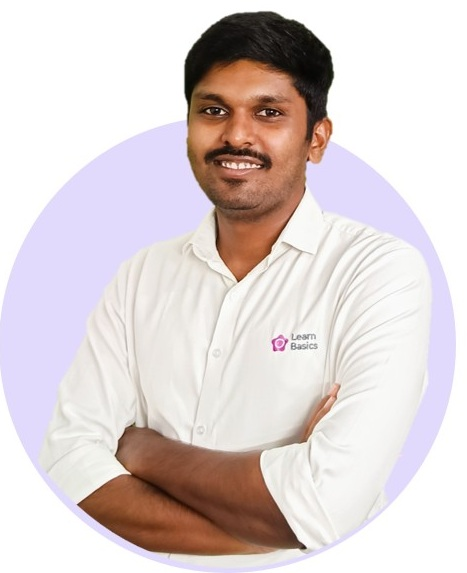
\includegraphics[width=1.5cm]{Saran Ravi.jpg}
\end{minipage}
\hspace{.5mm}
\begin{minipage}{4cm}
\vspace{6mm}
\renewcommand{\arraystretch}{.5}
\begin{tabular}{l}
    \textcolor{headingColor}{\textbf{Saran Ravi,} {\tiny(B.Tech.,NIT-T)}}\vspace{1pt} \\
    \textcolor{headingColor}{\footnotesize CTO \& Co-Founder}\\
\end{tabular}
\end{minipage}}

\newcommand{\prem}{\begin{minipage}{1.5cm} % Adjust the width as needed
    \centering
    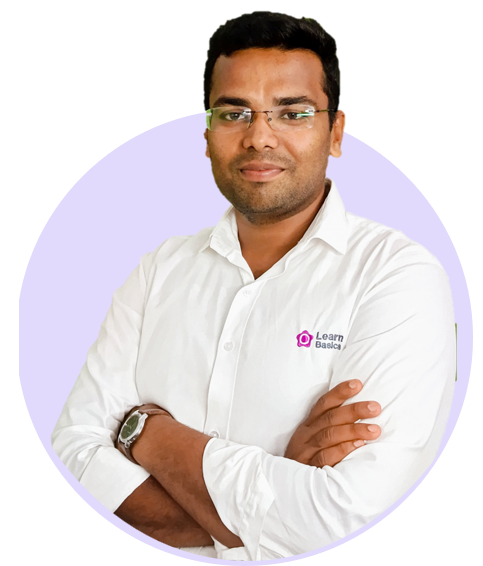
\includegraphics[width=1.5cm]{Prem kumar R.png}
\end{minipage}
\hspace{.5mm}
\begin{minipage}{4cm}
\vspace{6mm}
\renewcommand{\arraystretch}{.5}
\begin{tabular}{l}
    \textcolor{headingColor}{\textbf{Premkumar Ravichandran}}\vspace{1pt} \\
    \textcolor{headingColor}{\footnotesize CBO \& Co-Founder}\\
\end{tabular}
\end{minipage}}

\newcommand{\thaarun}{\begin{minipage}{1.5cm} % Adjust the width as needed
    \centering
    
\includegraphics[width=1.5cm]{Thaarun VG.png}
\end{minipage}
\hspace{.5mm}
\begin{minipage}{4.5cm}
\vspace{6mm}
\renewcommand{\arraystretch}{.5}
\begin{tabular}{l}
    \textcolor{headingColor}{\textbf{Thaarun VG}}\vspace{1pt}\\
    \textcolor{headingColor}{\footnotesize Co-Founder \& Program Director}\\
\end{tabular}
\end{minipage}
}

\newcommand{\aasha}{\begin{minipage}{1.5cm} % Adjust the width as needed
    \centering
    \vspace{5mm}
    \includegraphics[width=1.75cm]{Aasha.png}
\end{minipage}
\hspace{.5mm}
\begin{minipage}{4cm}
\vspace{6mm}
\renewcommand{\arraystretch}{.5}
\begin{tabular}{l}
    \textcolor{headingColor}{\textbf{Aasha Prabha}}\vspace{1pt} \\
    \textcolor{headingColor}{\footnotesize Program Associate}\\
\end{tabular}
\end{minipage}}

\newcommand{\nagarjun}{\begin{minipage}{1.5cm} % Adjust the width as needed
    \centering
    \vspace{5mm}
    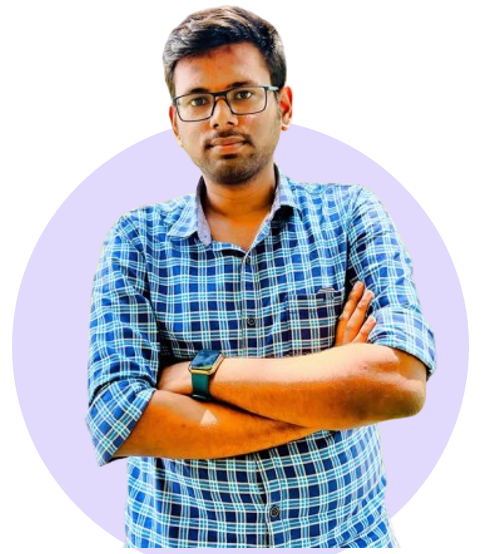
\includegraphics[width=1.75cm]{Nagarjun.png}
\end{minipage}
\hspace{.5mm}
\begin{minipage}{4cm}
\vspace{6mm}
\renewcommand{\arraystretch}{.5}
\begin{tabular}{l}
    \textcolor{headingColor}{\textbf{Nagarjun V}}\vspace{1pt} \\
    \textcolor{headingColor}{\footnotesize Program Associate}\\
\end{tabular}
\end{minipage}}